\documentclass[
	hyperref={
		pageanchor=false,
		bookmarks=false,
		pdfpagelabels=false},
	% aspectratio=169,
	]{beamer}
\usepackage{pgfpages}									% for producing notes
\setbeameroption{show notes on second screen}
% \usetheme[progressbar=frametitle]{metropolis}           % Use metropolis theme
\useinnertheme{metropolis}
\useoutertheme[progressbar=frametitle]{metropolis}
\usecolortheme{metropolis}
\definecolor{lightblue}{RGB}{0,190,255}					% Define colors of corporate design of University of Stuttgart
\definecolor{midblue}{RGB}{0,81,158}
\definecolor{anthrazit}{RGB}{62,68,76}
\setbeamercolor{alerted text}{fg=midblue}				% Set colors
%\setbeamercolor{normal text}{fg=anthrazit}
\usepackage{caption}									% Use \captionof
\usepackage{tikz}
\usetikzlibrary{shapes,arrows}
\usepackage{amsmath}									% Use of align which is assumer superior to eqnarray
\usepackage{tabularx}									% Needed for using align in tabular-environment
\usepackage{array}										% Center text in column with specified width
\newcolumntype{P}[1]{>{\centering\arraybackslash}p{#1}}
% \usepackage{colortbl}									% Specify \arrayrulecolor for use in timeline
 \usepackage{booktabs}									% Use of \toprule
 \usepackage{tabu}
\usepackage{halloweenmath}

% \title{Application of Crowdsourcing}
% \subtitle{Learning \& Feedback}
\title{Application: Learning \& Feedback}
\date{October 31, 2017 $\pumpkin$}
\author{Andreas Poppele, Hyungyu Shin}
% \institute{KIXLAB, Korea Advanced Institue of Science and Technology}
%\logo{\includegraphics{images/unistuttgart_logo_de.jpg}}

\usepackage[T1]{fontenc} % utf8 <- produce real utf8 characters
\usepackage[utf8]{inputenc} % utf8 <- accept utf8 input characters
\usepackage[english]{babel}
\usepackage{anyfontsize} % mute warnings?
\usepackage{silence} % Error / Warning filter
\usepackage{textcomp} % Fix font warning
\usepackage[numbers]{natbib} % use natbib for \citeauthor{} and Co.

\makeatletter % Enable footnotes without marker
\def\blfootnote{\gdef\@thefnmark{}\@footnotetext}
\makeatother
%---------------------------------
% Silence Warning
%---------------------------------
\WarningFilter{biblatex}{Patching footnotes failed}
\WarningFilter{beamerthememetropolis}{You need to compile with XeLaTeX or LuaLaTeX to use the Fira fonts}

\NoHyper % remove warnings - but no links


\begin{document}
	\maketitle

	\begin{frame}
		\frametitle{Outline}
		\tableofcontents
	\end{frame}
\setlength{\belowcaptionskip}{-1.5em}

%---------------------------------
% Section Problem Motivation
%---------------------------------
\section{First paper}
	\begin{frame}{First paper}
			\begin{itemize}
				\item<+-> Summarizing is a good way to memorize and understand
				\item<+-> Many students prepare summary (alone)
				\item<.-> ... and some don't
				\item<+-> Many summaries miss structure, are boring and possibly incomplete
			\end{itemize}
	\end{frame}

	\note{
		\begin{itemize}
			\item Boring: no colors, no images/drawings
			\item Structure: no relationship, no "Global Picture"
		\end{itemize}
	}

	\begin{frame}[standout]
		\begin{figure}
			\centering
			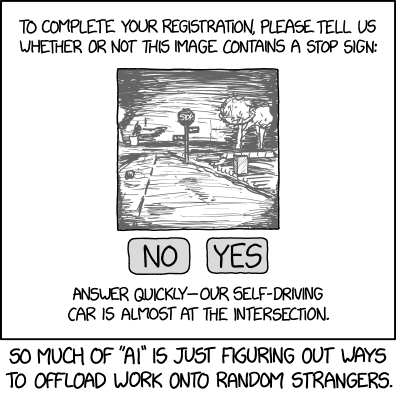
\includegraphics[width=0.7\textwidth]{images/self_driving}
			\label{fig:bad_note}
		\end{figure}
		xkcd.com
	\end{frame}

% \fontsize{6pt}{7.2}\selectfont
% \bibliographystyle{./aux/IEEEtranN}
% \bibliography{./aux/IEEEabrv,../ArbeitBib}

\end{document}
